% mnemonic-toolkit/docs/technical-manual/pandoc/preamble.tex
%
% LaTeX preamble passed to pandoc via `-H preamble.tex` for the PDF build.
% Authors should NOT edit individual chapters with raw LaTeX; only the
% directives loaded here (`\index{...}`, `:::primer` divs handled by Lua
% filter) are part of the authoring contract.

% --- Index support (book-style alphabetical index w/ page numbers) ---------
% Single load site: metadata.yaml's header-includes mechanism does not
% reliably round-trip raw LaTeX in pandoc 3.x without per-item raw-block
% wrappers, so we load + invoke makeidx here.
\usepackage{makeidx}
\makeindex

% --- Primer-box rendering for `:::primer` fenced divs ------------------------
\usepackage{mdframed}
\usepackage{xcolor}
\definecolor{primerbg}{RGB}{245,245,245}
\definecolor{primerrule}{RGB}{180,180,180}

\newmdenv[
  backgroundcolor=primerbg,
  linecolor=primerrule,
  linewidth=0.4pt,
  innertopmargin=6pt,
  innerbottommargin=6pt,
  innerleftmargin=10pt,
  innerrightmargin=10pt,
  skipabove=8pt,
  skipbelow=8pt,
]{primerbox}

% --- DANGER admonitions (used in worked-example chapters) --------------------
\definecolor{dangerbg}{RGB}{255,235,235}
\definecolor{dangerrule}{RGB}{180,40,40}

\newmdenv[
  backgroundcolor=dangerbg,
  linecolor=dangerrule,
  linewidth=1pt,
  innertopmargin=6pt,
  innerbottommargin=6pt,
  innerleftmargin=10pt,
  innerrightmargin=10pt,
  skipabove=8pt,
  skipbelow=8pt,
]{dangerbox}

% --- Better code-block typography -------------------------------------------
% Loaded here too. `-H preamble.tex` lands in `$for(header-includes)$`,
% which precedes `$highlighting-macros$` in pandoc's template — so this
% \DefineVerbatimEnvironment runs early enough to be authoritative.
% `commandchars=\\\{\}` is required for pandoc's syntax-highlighting
% commands (\ExtensionTok, \NormalTok, \AttributeTok, etc.) to expand
% inside the Verbatim environment; without it they render as literal text.
\usepackage{fvextra}
\DefineVerbatimEnvironment{Highlighting}{Verbatim}{
  commandchars=\\\{\},
  breaklines,
  breakanywhere,
  fontsize=\footnotesize,
}

% --- Mermaid figures (embedded as SVG by mermaid-filter) --------------------
\usepackage{graphicx}
\usepackage{svg}

% --- Title-page constellation graphic (m-format constellation) -----------------------
\usepackage{tikz}
\usetikzlibrary{shapes.geometric}
\usepackage{etoolbox}

\newcommand{\mformatconstellation}{%
  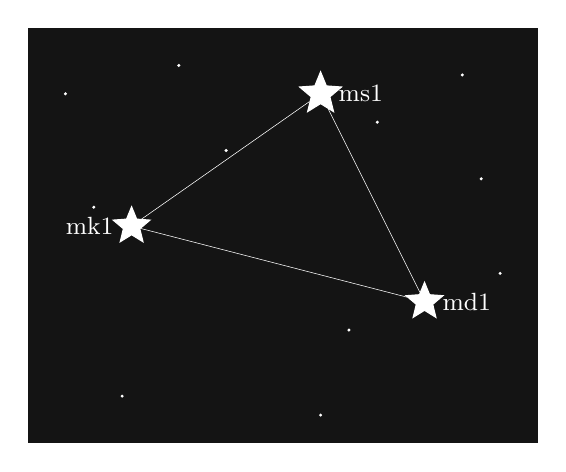
\begin{tikzpicture}[scale=1.2]
    \fill[black!92] (-2.7,-2.2) rectangle (2.7,2.2);
    % faint background stars
    \foreach \x/\y in {-2.3/1.5, -1.7/-1.7, -0.6/0.9, 0.4/-1.9, 1.9/1.7, 2.3/-0.4, 1.0/1.2, -2.0/0.3, 0.7/-1.0, -1.1/1.8, 2.1/0.6} {
      \fill[white] (\x,\y) circle (0.5pt);
    }
    % three labeled bright stars
    \node[star, star points=5, star point ratio=2.25, fill=white, draw=white, inner sep=2.5pt] (ms) at (0.4, 1.5) {};
    \node[right=3pt, white, font=\small] at (ms) {ms1};
    \node[star, star points=5, star point ratio=2.25, fill=white, draw=white, inner sep=2.2pt] (mk) at (-1.6, 0.1) {};
    \node[left=3pt, white, font=\small] at (mk) {mk1};
    \node[star, star points=5, star point ratio=2.25, fill=white, draw=white, inner sep=2.2pt] (md) at (1.5, -0.7) {};
    \node[right=3pt, white, font=\small] at (md) {md1};
    % connecting strokes
    \draw[white!55, very thin] (ms) -- (mk);
    \draw[white!55, very thin] (ms) -- (md);
    \draw[white!55, very thin] (mk) -- (md);
  \end{tikzpicture}%
}

% Inject the constellation below the title block (i.e., at the end of
% pandoc's titlepage environment, after \@title / \@author / \@date).
\AtEndEnvironment{titlepage}{%
  \vspace{2em}%
  \begin{center}\mformatconstellation\end{center}%
}

% --- Print the index at end (rendered into 99-zz-index location by Lua) -----
% Do not call \printindex here; the index is emitted by the index-anchor
% chapter (a stub markdown file containing only a raw-LaTeX block).
